% -*- root: ../Neurocomputacion.tex -*-
\section{Redes neuronales sencillas para clasificación de patrones}
\subsection{Redes Hebb}

\begin{problem}[1]
Apply the Hebb rule to the training patterns that define the XOR function.
\solution

Las \concept{redes neuronales Hebb} se caracterizan por la presencia de $n$ neuronas de entrada, una de salida y una neurona especial, conocida como ``bias'' que actúa como una neurona de entrada que siempre recibe el valor 1.

El entrenamiento de estas neuronas parte de la inicialización a 0 de todos los pesos de la red. Tras esto, y por cada vector de entrenamiento, ajustamos los pesos de la red según la ecuación:
\begin{equation}\label{eq:hebbRule}
w_i=w_i+x_iy
\end{equation}

siendo $y$ el valor esperado en la neurona de salida que estamos ajustando.

Si nuestra red tuviera varias neuronas de salida para cada una de ellas deberíamos aplicar el mismo procedimiento.

Ahora debemos ver como serán los datos de entrenamiento que definen la función XOR, que están recogidos en la siguiente tabla:
\begin{center}
\begin{tabular}{|c|c|c|}
\hline
\textbf{A} & \textbf{B} & \textbf{A XOR B}\footnote{Consideramos los valores de salida con una codificación bipolar ya que esta red no es capaz de aprender nada de aquellos patrones de entrenamiento con output nulo} \\
\hline
-1 & -1 & -1 \\
-1 & 1 & 1 \\
1 & -1 & 1 \\
1 & 1 & -1 \\
\hline
\end{tabular}
\end{center}

Es evidente ver que nuestra red tendrá un total de 4 neuronas siendo una de ellas la neurona de salida, por lo que nuestro vector de pesos inicializado será:
\[w = (0,0,0) \text{ siendo } w_0 \text{ el peso asociado al ``bias''}\]

Aplicando la ecuación \ref{eq:hebbRule} obtenemos el siguiente resultado:
\begin{center}
\begin{tabular}{|c|c|c|}
\hline
\textbf{Entrada} & \textbf{Vector de pesos antes} & \textbf{Vector de pesos despues} \\
$(x_1,x_2,y)$ & $(b,x_1,x_2)$ & $(b,x_1,x_2)$\\
\hline
(-1,-1,-1) & (0,0,0) & (-1,1,1)\\
(-1,1,1) & (-1,1,1) & (0,0,2)\\
(1,-1,1) & (0,0,2) & (1,1,1)\\
(1,1,-1) & (1,1,1) & (0,0,0)\\
\hline
\end{tabular}
\end{center}

No obtenemos un resultado válido puesto que la regla de Hebb sólo permite entrenar redes neuronales para problemas \concept{linealmente separables}, esto es, problemas en los que los puntos del espacio (en este caso un plano) que tienen salida positiva y los que tienen salida negativa pueden separarse linealmente.

En este caso concreto, los puntos a estudiar ocupan los vértices de un cuadrado siendo los vértices opuestos\footnote{Al hablar de vértices opuestos de un cuadrado nos referimos a vértices diagonalmente opuestos.} los que dan el mismo valor de salida. Evidentemente, no hay ninguna linea recta en el plano que separe vértices de un cuadrado en dos bloques dejando los opuestos en el mismo lado de la línea.


\end{problem}

\begin{problem}[2]
There are 16 different logic functions (with two inputs and one output), of which 14
are linearly separable. Show that the Hebb rule can find the weights for all problems
for which weights exist, as long as bipolar representation is used and a bias is included.

\solution

Las dos funciones lógicas que no pueden ser representadas mediante una red Hebb son el XOR y su negado.

La demostración de este hecho se basa en la idea comentada al final del ejercicio anterior. Si tenemos los 4 vértices de un cuadrado y queremos dividirlos en dos grupos por medio de una linea recta esta linea deberá, lógicamente, atravesar el cuadrado. Una vez comenzamos a dibujar la recta, esta deberá atravesar un lado del cuadrado, separando los dos vértices contiguos en distintos grupos.

Es evidente comprobar que no hay forma de prolongar esta recta (no importa que pendiente tomemos) de forma que los dos vértices restantes queden cada uno al lado de su opuesto.

La misma idea nos permite ver cláramente que cualquier otra selección de vértices de un cuadrado da lugar a un problema linealmente separable.

\end{problem}

\begin{problem}[3]
\ppart Consider character recognition using the Hebb rule. In Example 2.8, the "X" and
"0" used for training differed in all but four components. Show that the net will
respond correctly to an input vector formed from either the "X" or the "0" with
up to 20 components missing. (Whether it responds correctly, of course, is based on
your knowing which pattern you started with-you might prefer an "I don't know"
response. However, since the net input to the output unit is smaller the more components are missing, the "degree of certainty" of the response can also be judged.)

\ppart Mistakes involve one or more pixels switching from the value in the original
training pattern to the opposite value. Show that at approximately 10 mistakes, the
net will be seriously confused. (The exact number depends on whether any of the
mistakes occur in the pixels where the training patterns differ.)
Example 2.8 could be rephrased as an example of distinguishing the pattern X
from not-X (rather than specifically detecting X versus 0). Another pattern (for not X) that might be added to the net is:

\begin{center}
% TODO: Meter esta imagen.
%\includegraphics[width=0.3\textwidth]{img/pattern.png}
\end{center}

\ppart Find the new weights to store this pattern together with the two patterns used in
Example 2.8. (You can work from the weights in the example.) What does the bias
value tell you? How does the ability of the net to respond to noisy (missing or mis-
taken) data change as you add more patterns to the net? (You will probably need to
try more patterns of your own choosing in order to form a good conjecture to answer
this question.)

\solution


Atendiendo al ejemplo mencionado podemos observar que la idea consiste en escribir la cadena de símbolos que representa cada letra como un vector de 25 coordenadas, que será el input de nuestra red de Hebb.

Tras el breve proceso de entrenamiento (descrito en el ejemplo) se obtienen los pesos de las diferentes conexiones. Finalmente, podemos ver que la red considerará que ha leído una $X$ siempre que:
\[Σ = \begin{array}{ccccc}
2x_1& -2x_2 & -2x_3 & -2x_4 & +2x_5 +\\
-2x_6 & + 2x_7 &  & + 2x_9 &- 2x_{10} +\\
-2x_{11} & & +2x_{13} & & -2x_{15} + \\
-2x_{16} & +2x_{17} & & +2x_{19} & -2x_{20} + \\
+2x_{21} & -2x_{22} & -2x_{23} & -2x_{24} & +2x_{25} \\
\end{array} > 0\]

También nos indica el enunciado que, en caso de leer una $X$ perfecta, la suma anterior tiene valor $Σ=42$.

En esta ocasión, con la distribución de los pesos que acabamos de mostrar, las entradas que tendrán valor $1$ al leer la $X$ tienen pesos positivos y las que se activarán al leer el $O$ tienen valores negativos.

\spart
El primer apartado del problema nos pide comprobar que, aunque haya 20 casillas perdidas (es decir, 20 valores de entrada con valor 0), seguimos pudiendo detectar que se trataba de una $X$ (o de un $O$ respectivamente).

Basta con ver que cada \textbf{dato que nos falte}, salvo si es uno de los 4 valores asociados a un peso nulo, el valor de la neurona de salida decrece en dos unidades. Puesto que $Σ=42$, hasta 20 casillas sin información son toleradas, puesto que $Σ=42-2\cdot 20 > 0$\footnote{De hecho podrían faltar datos de incluso 24 casillas, si estas casillas son las adecuadas. No obstante, de forma general sólo podemos garantizar la correctitud de la red a la hora de clasificar el input si no faltan más de 20 datos}.

\spart
Por otro lado, es sencillo notar que un \textbf{fallo en un valor}, salvo en los casos en que el peso asociado a la neurona que lee ese valor es 0, implica una reducción en el valor de la neurona de salida de 4 unidades. Queda claro por tanto que $Σ=42-4\cdot 10>0$ por lo que hasta 10 errores son tolerados.

El mismo razonamiento partiendo de $Σ=-42$ que se ve aumentado con cada pérdida de información/error puede hacerse para el caso en que la entrada sea un $O$.

\spart
Vamos a completar ahora el entrenamiento de la red con el nuevo patrón que se nos proporciona. Recordando que el aprendizaje en las redes Hebb se lleva a cabo según la ecuación \ref{eq:hebbRule}, es sencillo comprobar que, tras el último paso del entrenamiento, tendremos:
\[Σ = -1 + \begin{array}{ccccc}
+3x_1& -1x_2 & -3x_3 & -1x_4 & +3x_5 +\\
-1x_6 & + 1x_7 & +x_8 & + 1x_9 &- 1x_{10} +\\
-1x_{11} & -x_{12} & +1x_{13} & -x_{14} & -1x_{15} + \\
-3x_{16} & +3x_{17} & +x_{18} & +3x_{19} & -3x_{20} + \\
+1x_{21} & -1x_{22} & -1x_{23} & -1x_{24} & +1x_{25} \\
\end{array}\]

Podemos comprobar que tras este entrenamiento el valor de la neurona de salida tras leer el patrón $X$ es $Σ=35$, con lo que se ha reducido la capacidad de detectar errores y fallos a la hora de clasificar el patrón $X$.

En general, a medida que añadamos patrones distintos de $X$ para el entrenamiento, habrá más distribuciones para las que el resultado Σ deba ser negativo. Por tanto cada vez menos ruido será necesario para hacer que la red clasifique mal un patrón $X$.
\end{problem}

\begin{problem}[4]
Create more letters, or different versions of X's and O's, for more training or testing
of the Hebb net.

\solution

Vamos a comprobar el resultado devuelto por la red al analizar los siguientes patrones:

\begin{center}
\begin{tabular}{|c|c|}
\hline
\textbf{Patrón} & \textbf{Clasificación} \\
\hline
 . \# \# \#  . & \\
\#  . \#  . \# & \\
\# \#  . \# \# & -35. No es una $X$\\
\#  . \#  . \# & \\
 . \# \# \#  . & \\
\hline
\#  .  .  .  . & \\
 . \#  .  .  . & \\
 .  . \#  .  . & 10. Se trata de una $X$ \\
 .  .  . \#  . & \\
 .  .  .  . \# & \\
\hline
\end{tabular}
\end{center}

\end{problem}

\begin{problem}[5]
\ppart Using the Hebb rule, find the weights required to perform the following classifications: Vectors (1, 1, 1, 1) and ( - 1, 1, - 1, -1) are members of the class (and
therefore have target value 1); vectors (1, 1, 1, - 1) and (1, - 1, - 1, 1) are not
members of the class (and have target value -1).
\ppart Using each of the training x vectors as input, test the response of the net.
\solution

\spart
El proceso de entrenamiento de la red, que se realiza según la fórmula \ref{eq:hebbRule} queda ilustrado en la siguiente tabla:

\begin{center}
\begin{tabular}{|c|c|c|c|c|c|}
\hline
\textbf{Input} & \textbf{Target} & \textbf{Pesos antes} & \textbf{Bias antes} & \textbf{Pesos después} & \textbf{Bias después} \\
\hline
(1,1,1,1)    & 1  & (0,0,0,0) & 0 & (1,1,1,1) & 1\\
(-1,1,-1,-1) & 1  & (1,1,1,1) & 1 & (0,2,0,0) & 2\\
(1,1,1,-1)   & -1 & (0,2,0,0) & 2 & (-1,1,-1,1) & -1\\
(1,-1,-1,1)  & -1 & (-1,1,-1,1) & -1 & (-2,2,0,0) & 0\\
\hline
\end{tabular}
\end{center}

\spart
Vamos a comprobar que el entrenamiento ha funcionado, para ello debemos comprobar que el producto escalar del vector de pesos por el traspuesto del input nos da un valor positivo para aquellos input de la primera clase y negativo para los de la segunda.

\begin{center}
\begin{tabular}{|c|c|c|}
\hline
\textbf{Input} & \textbf{Target} & \textbf{Resultado} \\
\hline
(1,1,1,1)    & 1  & 0 \\
(-1,1,-1,-1) & 1  & 4 \\
(1,1,1,-1)   & -1 & 0 \\
(1,-1,-1,1)  & -1 & -4 \\
\hline
\end{tabular}
\end{center}

Podemos concluir que no se trata de un problema lineal puesto que el entrenamiento no da un resultado satisfactorio ni si quiera para los propios datos de entrenamiento.

\end{problem}

\begin{problem}[6]
\ppart The Hebb rule is sometimes used by converting the binary training patterns (inputs
and targets) to bipolar form to find the weight matrix. Apply this procedure to
find the weights to store the following classifications:
\begin{center}
s(1) = (1,0, 1), t(1) = 1\\
s(2) = (1, 1,0), t(2) = 0
\end{center}
\ppart Using the binary step function (with threshold 0) as the output unit's activation
function, test the response of your network on each of the binary training patterns.
\ppart Using the bipolar step function (with threshold 0) as the output unit's activation
function, convert the training patterns to bipolar form and test the network response again.
\ppart Test the response of your network on each of the following noisy versions of the
bipolar form of the training patterns:
\begin{center}
(0,-1,1) (0, 1, -1) (0, 0, 1) (0,0, -1) (0, 1,0) (0, -1,0)\\
(1, 0, 1) (1,0, -1) (1, -1,0) (1,0, 0) (1, 1,0) (1, 1, 1)
\end{center}
Which of the responses are correct, which are incorrect, and which are indefinite
(undetermined)?

\solution
\spart
Una vez más procedemos a entrenar una red de Hebb basándonos en datos de entrenamiento dados en forma bipolar. El resultado queda recogido en la siguiente tabla:
\begin{center}
\begin{tabular}{|c|c|c|c|c|c|}
\hline
\textbf{Input} & \textbf{Target} & \textbf{Pesos antes} & \textbf{Bias antes} & \textbf{Pesos después} & \textbf{Bias después} \\
\hline
(1,-1,1) & 1  & (0,0,0) & 0 & (1,-1,1) & 1\\
(1,1,-1) & -1 & (1,-1,1) & 1 & (0,-2,2) & 0\\
\hline
\end{tabular}
\end{center}

\spart
La red que acabamos de crear opera sobre los input dados (en binario) como muestra la siguiente tabla
\begin{center}
\begin{tabular}{|c|c|c|c|}
\hline
\textbf{Input} & \textbf{Target} & \textbf{Resultado} & \textbf{Clasificación}\\
\hline
(1,0,1) & 1  & 2 & 1\\
(1,1,0) & 0 & -2 & 0\\
\hline
\end{tabular}
\end{center}
Con lo que parece que el resultado obtenido es satisfactorio.

\spart
Operando sobre los datos de entrada en formato bipolar tenemos:
\begin{center}
\begin{tabular}{|c|c|c|c|}
\hline
\textbf{Input} & \textbf{Target} & \textbf{Resultado} & \textbf{Clasificación}\\
\hline
(1,-1,1) & 1 &  4 & 1\\
(1,1,-1) & 0 & -4 & -1\\
\hline
\end{tabular}
\end{center}
Con lo que parece que el resultado obtenido es satisfactorio.

\spart
Operando sobre los datos de entrada en formato bipolar tenemos:
\begin{center}
\begin{tabular}{|c|c|c|c|}
\hline
\textbf{Input} & \textbf{Target} & \textbf{Resultado} & \textbf{Clasificación}\\
\hline
(0,-1,1)   &  1 & 4  & 1\\
(0, 1, -1) & -1 & -4  & -1\\
(0, 0, 1)  &  1 & 2  & 1\\
(0,0, -1)  & -1 & -2 & -1\\
(0, 1,0)   & -1 & -2 & -1\\
(0, -1,0)  &  1 & 2 & 1\\
(1, 0, 1)  &  1 & 2 & 1\\
(1,0, -1)  & -1 & -2 & -1\\
(1, -1,0)  &  1 & 2 & 1\\
(1,0, 0)   &  ? & 0  & 1\\
(1, 1,0)   & -1 & -2 & -1\\
(1, 1, 1)  &  ? & 0 & 1\\
\hline
\end{tabular}
\end{center}

Los resultados esperados (columna Target) los he deducido buscando el vecino más próximo. Podemos comprobar que los resultados esperados coinciden exactamente con los obtenidos salvo, lógicamente, en los casos donde no hay un resultado esperado claro.

\end{problem}

\subsection{Perceptrón}

\begin{problem}[7]
Graph the changes in separating lines as they occur in Example 2.12.
\solution

Puesto que en esta ocasión el umbral es $\theta = 0$ sólo tendremos que dibujar una linea en cada iteración.

Por comodidad copiamos aquí la tabla que aparece en el ejemplo indicado, que recoge la evolución de los pesos de un perceptrón que está siendo entrenado para reconocer la función AND. El entrenamiento se realiza con entradas y salidas bipolares.


\begin{minipage}{0.4\textwidth}
\begin{center}
\begin{tabular}{|c|ccc|}
\hline
\textbf{Iteración} & & \textbf{Pesos} & \\
& $ω_1$ & $ω_2$ & $b$ \\
\hline
1 & 1 & 1 & 1\\
\hline
2 & 0 & 2 & 0\\
\hline
3 & 1 & 1 & -1\\
\hline
4 & 1 & 1 & -1\\
\hline
5 & 1 & 1 & -1\\
\hline
6 & 1 & 1 & -1\\
\hline
7 & 1 & 1 & -1\\
\hline
8 & 1 & 1 & -1 \\
\hline
\end{tabular}
\end{center}
\end{minipage}
\begin{minipage}{0.58\textwidth}
\begin{center}
\begin{tikzpicture}
\begin{axis}[
axis y line=center,
axis x line=middle,
axis equal,
grid=none,
xmax=5,xmin=-5,
ymin=-5,ymax=5,
xlabel=$ω_1$,ylabel=$ω_2$,
xtick=\empty,
ytick=\empty,
width=10cm,
anchor=center,
]
\addplot[no marks, color=red, very thick] {-x-1} ;
\addplot[no marks, color=blue, very thick] {0} ;
\addplot[no marks, color=green, very thick] {-x+1} ;
\addlegendentry{Iteración 1}
\addlegendentry{Iteración 2}
\addlegendentry{Iteración >3}
\end{axis}
\end{tikzpicture}
\end{center}
\end{minipage}

En los tres casos representados, el semiplano de aceptación es el que se encuentra por encima de la linea divisoria.
\end{problem}

\begin{problem}[8]
Explore the influence of the value of the learning rate on the speed of convergence
of perceptron learning:
\ppart Consider different values of α in Example 2.12; explain your results.
\ppart Modify the proof of the perceptron learning rule convergence theorem to include
an arbitrary learning rate α.
\solution

\spart

El ejemplo 2.12 se caracteriza por el empleo de un umbral $\theta = 0$. En este caso concreto, la modificación del valor α no tiene ningún efecto en la velocidad de convergencia del proceso de aprendizaje.

Para convencerse de ello basta con observar que lo único que nos importa es si el valor de salida de la red es mayor, menor o igual que 0. Puesto que empezamos con los pesos inicializados a 0, el efecto de cambiar α por un valor distinto simplemente modifica el valor neto obtenido en cada iteración pero no altera en absoluto la salida bipolar de la red.

La tabla representada en el ejemplo seguiría siendo la misma aunque los pesos aparecerían multiplicados por α, sea cual sea su valor (considerándolo siempre positivo)

\spart

Vamos a imitar la demostración del libro con el cambio dado en el enunciado.

Consideramos, como se hace en la demostración del libro, el conjunto de entrenamiento, $F$, formado por lo patros de entrenamiento con salida esperada $1$ y la negación de los patrones de entrenamiento con salida esperada $-1$. Así, todos los patrones de $F$ tienen salida esperada $1$.

Definimos como $\vec{w}^*$ el vector de pesos solución, cuya existencia suponemos. Así:
\begin{equation}\label{eq:vectorPesosSol}
\forall \vx \in F, \ \vec{w}^*\cdot \vx > 0
\end{equation}

Empezamos con un vector de pesos nulo $\vec{w}(0)=\vec{0}$. Con cada patrón de entrenamiento, si se produce un error la modificación producida sobre los pesos, esta será de la forma:
\[\vec{w}(i) = \vec{w}(i-1)+α\cdot \vx(i-1)\]

Cuando iteremos sobre todos los patrones de entrenamiento tendremos:
\[\vec{w}(k) = \vec{w}(0) + α\cdot \sum_{i=0}^{k-1} \vec{w}(i)\]
donde estamos iterando sobre aquellos patrones de entrenamiento que produjeron un error.

De la ecuación \ref{eq:vectorPesosSol}, sabiendo que el conjunto de patrones de entrenamiento es finito, podemos deducir que existe
\[m=\min\{\vx \cdot \vec{w}^*\}\]
La existencia de este mínimo nos permite escribir:
\[\vec{w}(k)\cdot \vec{w}^* = \vec{w}(0)\cdot \vec{w}^*+αkm\]
puesto que $\vx(i)\cdot \vec{w}^* \geq m \ \forall i$.

Empleando ahora la desigualdad de Cauchy-Schwartz podemos escribir
\begin{equation}\label{eq:Dif1}
\norm{\vec{w}(k)}^2 \geq \frac{(\vec{w}(k)\cdot \vec{w}^*)^2}{\norm{\vec{w}^*}^2} \geq  \frac{(\vec{w}(0)\cdot \vec{w}^*+αkm)^2}{\norm{\vec{w}^*}^2}
\end{equation}

Ahora vamos a comprobar que el valor $k$ no puede ser arbitrariamente grande. Consideramos
\[\vec{w}(k)=\vec{w}(k-1)+\vx(k-1)\]
sabiendo que
\[\vx(k-1)\cdot \vec{w}(k-1) \leq 0\]
podemos ver que
\[\norm{\vec{w}(k)}^2 \leq \norm{\vec{w}(k-1)}^2 + \norm{\vx(k-1)}^2\]

Siendo $M=\max_{\vx \in F}\{\norm{\vx}^2\}$ tenemos

\begin{equation}\label{eq:Dif2}
\begin{array}{lll}
\norm{\vec{w}(k)}^2 & \leq & \norm{\vec{w}(k-1)}^2+\norm{\vx(k-1)}^2\\
 & \leq & \norm{\vec{w}(k-2)}^2 + \norm{\vx(k-2)}^2 + \norm{\vx(k-1)}^2\\
 & & \vdots \\
 & \leq & \norm{\vec{w}(0)}^2 + \norm{\vx(0)}^2 + \cdots + \norm{\vx(k-1)}^2\\
 & \leq & \norm{\vec{w}(0)}^2 + kM
\end{array}
\end{equation}

Combinando las desigualdades \ref{eq:Dif1} y \ref{eq:Dif2} y considerando que el vector de pesos inicial es nulo tenemos
\[\frac{(αkm)^2}{\norm{\vec{w}^*}^2} \leq k M \implies k \leq \frac{M\norm{\vec{w}^*}^2}{m^2α}\]

\end{problem}

\begin{problem}[9]
 Show that the use of a bias is essential in Example 2.11. That is, show that it is
impossible to find weights W I and W2 for which the points (1,1), (1,0), (0,1), and (0,0)
are classified correctly. First, show that (0,0) will never be classified correctly, and
in fact, no learning will ever occur for that point. Then, neglecting (0,0), consider
whether (1,1), (1,0), and (0,1) can be classified correctly. That is, do weights WI and
W2 exist such that
\begin{center}
(1)$w_1$ + (1)$w_2$ > $\theta $ > 0,\\
(1)$w_1$ + (0)$w_2$ < $-\theta $ < 0,\\
(0)$w_1$ + (1)$w_2$ < $-\theta $ < 0
\end{center}
\solution

Sin tuviéramos $b=0$, tal y como está descrito el ejemplo 2.11, tendríamos siempre dos rectas de la forma:
\[y_1=ax+0.2 \text{ y } y_2 = bx - 0.2\]

El punto $(0,0)$ cumplirá siempre $y_1>0$ y $y_2<0$ por lo que no podrá ser clasificado correctamente.

Obviando este problema, vamos a ver qué ocurre con los otros puntos. Si existieran los valores $a$ y $b$ que dan lugar a las rectas descritas anteriormente, tendríamos:
\[\begin{array}{l}
1 > a+0.2 \\
1 > b-0.2 \\
a+0.2 > 0 \\
b-0.2 > 0 \\
0.2 > 1 \\
-0.2 > 1\\
\end{array}\]
donde las ecuaciones se obtienen al forzar que los puntos $(1,1), (1,0)$ y $(0,1)$ tengan los signos adecuados.

Finalmente, aunque las cuatro primeras ecuaciones dan lugar a la posibilidad de existir las rectas $y_1$ y $y_2$\footnote{Como es lógico puesto que si ignoramos el origen y uno de los puntos que se encuentran sobre los ejes es trivial ver que toda recta con pendiente menor que 1 (o mayor, según que punto del eje estemos ignorando) actúa como linea divisoria}, las dos últimas ecuaciones son inconsistentes.

\end{problem}

\begin{problem}[10]
Show that small initial weights still allow for any position of the initial decision line
for the perceptron.

\solution



\end{problem}

\begin{problem}[11]
 Repeat Example 2.11, and show that there is no change in the training process if
$\theta = 0$. Show that the separating line is
\[x_2=-\frac{2}{3}x_1+\frac{4}{3}\]
\solution

Es evidente que el cambio en el valor de $\theta$ indicado no cambia nada puesto que el valor calculado por la red, así como los pesos van a tener siempre valores enteros. Por tanto el único valor calculado por la red que de lugar a un output de 0 es el propio 0. Para el resto de valores calculados por la red, el output coincidirá con el signo del valor calculado.

Vamos a constuir la tabla correspondiente para ver cómo se comporta la red con $\theta = 0$

\begin{center}
\begin{tabular}{|c|c|c|c|c|c|c|}
\hline
\textbf{Input} & \textbf{Pesos antes} &  \textbf{Bias antes} & \textbf{Out} & \textbf{Target} & \textbf{Pesos después} & \textbf{Bias después} \\
\hline
( 1 , 1 , 1 ) & ( 0 , 0 ) &  0  &  0  &  1  & ( 1 , 1 ) &  1  \\
( 1 , 0 , 1 ) & ( 1 , 1 ) &  1  &  1  &  -1  & ( 0 , 1 ) &  0  \\
( 0 , 1 , 1 ) & ( 0 , 1 ) &  0  &  1  &  -1  & ( 0 , 0 ) &  -1  \\
( 0 , 0 , 1 ) & ( 0 , 0 ) &  -1  &  -1  &  -1  & ( 0 , 0 ) &  -1  \\
( 1 , 1 , 1 ) & ( 0 , 0 ) &  -1  &  -1  &  1  & ( 1 , 1 ) &  0  \\
( 1 , 0 , 1 ) & ( 1 , 1 ) &  0  &  1  &  -1  & ( 0 , 1 ) &  -1  \\
( 0 , 1 , 1 ) & ( 0 , 1 ) &  -1  &  0  &  -1  & ( 0 , 0 ) &  -2  \\
( 0 , 0 , 1 ) & ( 0 , 0 ) &  -2  &  -1  &  -1  & ( 0 , 0 ) &  -2  \\
( 1 , 1 , 1 ) & ( 0 , 0 ) &  -2  &  -1  &  1  & ( 1 , 1 ) &  -1  \\
( 1 , 0 , 1 ) & ( 1 , 1 ) &  -1  &  0  &  -1  & ( 0 , 1 ) &  -2  \\
( 0 , 1 , 1 ) & ( 0 , 1 ) &  -2  &  -1  &  -1  & ( 0 , 1 ) &  -2  \\
( 0 , 0 , 1 ) & ( 0 , 1 ) &  -2  &  -1  &  -1  & ( 0 , 1 ) &  -2  \\
( 1 , 1 , 1 ) & ( 0 , 1 ) &  -2  &  -1  &  1  & ( 1 , 2 ) &  -1  \\
( 1 , 0 , 1 ) & ( 1 , 2 ) &  -1  &  0  &  -1  & ( 0 , 2 ) &  -2  \\
( 0 , 1 , 1 ) & ( 0 , 2 ) &  -2  &  0  &  -1  & ( 0 , 1 ) &  -3  \\
( 0 , 0 , 1 ) & ( 0 , 1 ) &  -3  &  -1  &  -1  & ( 0 , 1 ) &  -3  \\
( 1 , 1 , 1 ) & ( 0 , 1 ) &  -3  &  -1  &  1  & ( 1 , 2 ) &  -2  \\
( 1 , 0 , 1 ) & ( 1 , 2 ) &  -2  &  -1  &  -1  & ( 1 , 2 ) &  -2  \\
( 0 , 1 , 1 ) & ( 1 , 2 ) &  -2  &  0  &  -1  & ( 1 , 1 ) &  -3  \\
( 0 , 0 , 1 ) & ( 1 , 1 ) &  -3  &  -1  &  -1  & ( 1 , 1 ) &  -3  \\
( 1 , 1 , 1 ) & ( 1 , 1 ) &  -3  &  -1  &  1  & ( 2 , 2 ) &  -2  \\
( 1 , 0 , 1 ) & ( 2 , 2 ) &  -2  &  0  &  -1  & ( 1 , 2 ) &  -3  \\
( 0 , 1 , 1 ) & ( 1 , 2 ) &  -3  &  -1  &  -1  & ( 1 , 2 ) &  -3  \\
( 0 , 0 , 1 ) & ( 1 , 2 ) &  -3  &  -1  &  -1  & ( 1 , 2 ) &  -3  \\
( 1 , 1 , 1 ) & ( 1 , 2 ) &  -3  &  0  &  1  & ( 2 , 3 ) &  -2  \\
( 1 , 0 , 1 ) & ( 2 , 3 ) &  -2  &  0  &  -1  & ( 1 , 3 ) &  -3  \\
( 0 , 1 , 1 ) & ( 1 , 3 ) &  -3  &  0  &  -1  & ( 1 , 2 ) &  -4  \\
( 0 , 0 , 1 ) & ( 1 , 2 ) &  -4  &  -1  &  -1  & ( 1 , 2 ) &  -4  \\
( 1 , 1 , 1 ) & ( 1 , 2 ) &  -4  &  -1  &  1  & ( 2 , 3 ) &  -3  \\
( 1 , 0 , 1 ) & ( 2 , 3 ) &  -3  &  -1  &  -1  & ( 2 , 3 ) &  -3  \\
( 0 , 1 , 1 ) & ( 2 , 3 ) &  -3  &  0  &  -1  & ( 2 , 2 ) &  -4  \\
( 0 , 0 , 1 ) & ( 2 , 2 ) &  -4  &  -1  &  -1  & ( 2 , 2 ) &  -4  \\
( 1 , 1 , 1 ) & ( 2 , 2 ) &  -4  &  0  &  1  & ( 3 , 3 ) &  -3  \\
( 1 , 0 , 1 ) & ( 3 , 3 ) &  -3  &  0  &  -1  & ( 2 , 3 ) &  -4  \\
( 0 , 1 , 1 ) & ( 2 , 3 ) &  -4  &  -1  &  -1  & ( 2 , 3 ) &  -4  \\
( 0 , 0 , 1 ) & ( 2 , 3 ) &  -4  &  -1  &  -1  & ( 2 , 3 ) &  -4  \\
( 1 , 1 , 1 ) & ( 2 , 3 ) &  -4  &  1  &  1  & ( 2 , 3 ) &  -4  \\
( 1 , 0 , 1 ) & ( 2 , 3 ) &  -4  &  -1  &  -1  & ( 2 , 3 ) &  -4  \\
( 0 , 1 , 1 ) & ( 2 , 3 ) &  -4  &  -1  &  -1  & ( 2 , 3 ) &  -4  \\
( 0 , 0 , 1 ) & ( 2 , 3 ) &  -4  &  -1  &  -1  & ( 2 , 3 ) &  -4  \\

\hline
\end{tabular}
\end{center}

Una vez hemos realizado todo el proceso de aprendizaje, es sencillo obtener la linea divisoria como:
\[x_1+3x_2-4 = 0 \implies x_2 = \frac{2}{3}x_1+\frac{4}{3}\]

\end{problem}

\begin{problem}[12]
 Consider carefully the difference in what can be solved using the following activation
functions:
\[f=\left\{ \begin{array}{ll}1 & \text{ if net } \geq \theta \\ 0 & \text{otherwise} \end{array}\right.\]
or
\[f=\left\{ \begin{array}{ll}1 & \text{ if net } \geq \theta \\ -1 & \text{otherwise} \end{array}\right.\]
or
\[f=\left\{ \begin{array}{ll}1 & \text{ if net } \geq \theta \\ 0 & \text{if} -\theta < \text{net} < \theta \\ -1 & \text{ if net } \leq -\theta\end{array}\right.\]
\solution

Considerando que estamos trabajando con un perceptrón (no lo especifica el enunciado pero estamos en la sección de problemas asociados al perceptrón) tendremos una función de activación (una vez hayamos entrenado la red) de la forma:
\[y = f\left(ω_0b + \sum_{i=1}^nω_ix_i\right) \]

Con las dos primeras funciones proporcionadas podemos resolver exactamente los mismos problemas. Lo que cambia es la codificación de la clasificación negativa por parte de la red. En estos casos podremos resolver todos aquellos problemas que sean linealmente separables.

En cuanto a la tercera función tendremos que los puntos estudiados se clasifican en tres tipos, según el valor de la neurona de salida respecto al umbral establecido. Esto nos permite resolver todos aquellos problemas que puedan separarse mediante dos rectas paralelas.

Por ejemplo, la función XOR, que no es separable, puede ser representada por un perceptrón que emplee una función como la tercera dada. Para ello basta con asociar la salida 1 y la salida -1 con la misma clasificación del patrón entrenado.

En el caso de la puerta lógica XOR que acabamos de mencionar tendríamos como solución:
\[y=f(-b + x_1+x_2) \text{ siendo } \theta =0.5\]

\end{problem}

\begin{problem}[13]
 Even for $\theta= 0$, the perceptron learning rule prevents the correct classification of a point on the dividing line (which is better than assigning it arbitrarily to either side
of the line). If $\theta < α$ (the learning rate), does the exact value of $\theta$ matter? Does it matter if $\theta > α?$ Does it make a difference whether we start with all initial weights
equal to 0, as in Examples 2.11-2.13, or with other values (small random numbers,
for instance)?

\solution

El proceso de aprendizaje del perceptrón consiste en reajustar los pesos de la red \textbf{cuando se produzca un error en la predicción} según la fórmula:
\[ω_i = ω_i + αtx_i, \text{ siendo } t \text{ la salida esperada}\]

Esta regla sólo se aplica en los siguientes casos:
\[\begin{array}{lll}
\sum_{i=0}^nω_ix_i < -\theta & \text{ y } & t\geq 0 \\
\theta \geq \sum_{i=0}^nω_ix_i \geq - \theta & \text{ y } & \abs{t}> 0 \\
\sum_{i=0}^nω_ix_i > \theta & \text{ y } & t\leq 0
\end{array}\]

Podemos obviar aquellos casos en los que $t=0$ puesto que en esos casos no se produce ningún aprendizaje por lo que las preguntas planteadas por el enunciado carecen de sentido.

En el primer caso, tras corregir los pesos, ante la misma entrada, tendremos:
\[\sum_{i=0}^nω_ix_i + \sum_{i=0}^nαtx_i^2 \]
siendo
\[ \theta  k\leq  \sum_{i=0}^nαtx_i^2 \leq  αk\]
donde $k$ es el número de valores $x_i$ no nulos.

\textcolor{red}{No se cómo seguir a partir de aquí. Supongo que hay que jugar con estas desigualdades pero no se qué más hacer.}
\end{problem}

\begin{problem}[14]
 A variation of the perceptron learning rule allows active input units to increase their
weights and inactive units to decrease their weights in such manner that the total
weights are constant [see Block, 1962, p. 144, footnote 50]. Consider the effect this
would have on the binary representation of the AND function in Example 2.11.

\solution

Según el libro: ``Principles of Neurodynamics'' un sistema de aprendizaje como el descrito en el enunciado es un sistema \textbf{gamma}, que se define en el libro como sigue:

\begin{defn}[Sistema Gamma]
El sistema de aprendizaje gamma es una regla que dicta cómo modificar los pesos de las conexiones que llegan a una determinada neurona de tal forma que a todas las conexiones activas sufren la misma variación manteniendo la suma total de las conexiones constante.

Por tanto, la misma cantidad total que se ha sumado se divide entre la cantidad de neuronas inactivas y se resta a cada conexión lo correspondiente.

La fórmula empleada es:
\[Δ ω_{ij}(t)=\left(v_{ij}(t)-\frac{\sum_i v_{ij}(t)}{N_j}\right)α\]
donde $v_{ij}(t)$ tiene valor $1$ si la conexión estaba activada en el instante $t$ y $0$ en caso contrario. $N_j$ es el número de conexiones que llegan a la neurona que estamos estudiando.
\end{defn}

\begin{center}
\begin{tabular}{|c|c|c|c|c|c|c|}
\hline
\textbf{Input} & \textbf{Pesos antes} &  \textbf{Bias antes} & \textbf{Out} & \textbf{Target} & \textbf{Pesos después} & \textbf{Bias después} \\
\hline
(1,1,1) & (0.34,0.42) & 0.085 & 1 & 1 & (0.34,0.42) & 0.085\\
(1,0,1) & (0.34,0.42) & 0.085 & 1 & -1 & (0.0067,1.0867) & -0.248\\
(0,1,1) & (0.0067,1.0867) & -0.248 & 1 & -1 & (0.67,0.75) & -0.58167\\
(0,0,1) & (0.67,0.75) & -0.58167 & -1 & -1 & (0.67,0.75) & -0.58167\\
(1,1,1) & (0.67,0.75) & -0.58167 & 1 & 1 & (0.67,0.75) & -0.58167\\
(1,0,1) & (0.67,0.75) & -0.58167 & 0 & -1 & (0.34,1.42) & -0.915\\
(0,1,1) & (0.34,1.42) & -0.915 & 1 & -1 & (1.0067,1.0867) & -1.248\\
(0,0,1) & (1.0067,1.0867) & -1.248 & -1 & -1 & (1.0067,1.0867) & -1.248\\
(1,1,1) & (1.0067,1.0867) & -1.248 & 1 & 1 & (1.0067,1.0867) & -1.248\\
(1,0,1) & (1.0067,1.0867) & -1.248 & -1 & -1 & (1.0067,1.0867) & -1.248\\
(0,1,1) & (1.0067,1.0867) & -1.248 & 0 & -1 & (1.67,0.75) & -1.58167\\
(0,0,1) & (1.67,0.75) & -1.58167 & -1 & -1 & (1.67,0.75) & -1.58167\\
(1,1,1) & (1.67,0.75) & -1.58167 & 1 & 1 & (1.67,0.75) & -1.58167\\
(1,0,1) & (1.67,0.75) & -1.58167 & 0 & -1 & (1.34,1.42) & -1.915\\
(0,1,1) & (1.34,1.42) & -1.915 & -1 & -1 & (1.34,1.42) & -1.915\\
(0,0,1) & (1.34,1.42) & -1.915 & -1 & -1 & (1.34,1.42) & -1.915\\
(1,1,1) & (1.34,1.42) & -1.915 & 1 & 1 & (1.34,1.42) & -1.915\\
(1,0,1) & (1.34,1.42) & -1.915 & -1 & -1 & (1.34,1.42) & -1.915\\
(0,1,1) & (1.34,1.42) & -1.915 & -1 & -1 & (1.34,1.42) & -1.915\\
(0,0,1) & (1.34,1.42) & -1.915 & -1 & -1 & (1.34,1.42) & -1.915\\

\hline
\end{tabular}
\end{center}

Por la propia definición de la regla, es claro que debemos establecer los pesos iniciales de manera aleatoria puesto que si inicializamos todos a $0$, nunca podríamos predecir adecuadamente el valor de la puerta AND, ya que en el único caso en que debe vale $1$ obtendríamos 0.

En este caso se ha tomado un valor α=-1, decisión tomada debido a las pruebas realizadas con resultados erróneos.
\end{problem}

\begin{problem}[15]
 Using the perceptron learning rule, find the weights required to perform the following
classifications: Vectors (1, 1, 1, 1) and ( - 1, 1, - 1, - 1) are members of the class
(and therefore have target value 1); vectors (1 , 1, 1, -1) and (1, - 1, - 1, 1) are not
members of the class (and have target value -1) . Use a learning rate of 1 and starting
weights of 0. Using each of the training x vectors as input, test the response of the
net.

\solution

Aplicando la regla, que aparece explicada en el libro a modo de pseudocódigo, para el aprendizaje del perceptrón obtenemos el resultado que recoge la siguiente tabla:

\begin{center}
\begin{tabular}{|c|c|c|c|c|c|c|}
\hline
\textbf{Input} & \textbf{Pesos antes} &  \textbf{Bias antes} & \textbf{Out} & \textbf{Target} & \textbf{Pesos después} & \textbf{Bias después} \\
\hline
(1,1,1,1) & (0,0,0,0) & 0 & 0 & 1 & (1,1,1,1) & 1\\
(-1,1,-1,-1) & (1,1,1,1) & 1 & -1 & 1 & (0,2,0,0) & 0\\
(1,1,1,-1) & (0,2,0,0) & 0 & 1 & -1 & (-1,1,-1,1) & 1\\
(1,-1,-1,1) & (-1,1,-1,1) & 1 & 0 & -1 & (-2,2,0,0) & 0\\
(1,1,1,1) & (-2,2,0,0) & 0 & 0 & 1 & (-1,3,1,1) & 1\\
(-1,1,-1,-1) & (-1,3,1,1) & 1 & 1 & 1 & (-1,3,1,1) & 1\\
(1,1,1,-1) & (-1,3,1,1) & 1 & 1 & -1 & (-2,2,0,2) & 2\\
(1,-1,-1,1) & (-2,2,0,2) & 2 & -1 & -1 & (-2,2,0,2) & 2\\
(1,1,1,1) & (-2,2,0,2) & 2 & 1 & 1 & (-2,2,0,2) & 2\\
(-1,1,-1,-1) & (-2,2,0,2) & 2 & 1 & 1 & (-2,2,0,2) & 2\\
(1,1,1,-1) & (-2,2,0,2) & 2 & -1 & -1 & (-2,2,0,2) & 2\\
(1,-1,-1,1) & (-2,2,0,2) & 2 & -1 & -1 & (-2,2,0,2) & 2\\
\hline
\end{tabular}
\end{center}

Podemos observar que en tres épocas la red ha sido capaz de encontrar la solución.
\end{problem}

\subsection{Adaline y Madaline}
\begin{problem}[16]
Repeat Examples 2.18 and 2.19 using binary rather than bipolar vectors
\solution

La idea de la red de Adaline es encontrar los pesos que minimizan el error cuadrático medio. Para ello lo que hacemos es escribir la fórmula del error cuadrático y derivar para buscar el gradiente, que nos da la dirección de máximo crecimiento.

Al escribir el error cuadrático medio, nuestras incógnitas son los pesos y es respecto a ellos como derivamos. El resultado nos da la dirección de máximo crecimiento, es decir, la forma en que se debe de variar los pesos para llegar al mínimo de la función.

Apoyándose en esta idea es sencillo llegar al algoritmo que describe el proceo de aprendizaje de las redes Adaline. Aplicando el algoritmo a los problemas mencionados obtenemos las siguientes soluciones:

\begin{itemize}
\item Función lógica AND NOT usando entradas binarias.


\begin{center}
\begin{tabular}{|c|c|c|c|c|c|c|}
\hline
\textbf{Input} & \textbf{Pesos antes} &  \textbf{Bias antes} & \textbf{Out} & \textbf{Target} & \textbf{Pesos después} & \textbf{Bias después} \\
\hline
(1,1,1) & (0.48,0.295) & 0.055 & 1 & -1 & (-1.35,-1.535) & -1.775\\
(1,0,1) & (-1.35,-1.535) & -1.775 & -1 & 1 & (2.775,-1.535) & 2.35\\
(0,1,1) & (2.775,-1.535) & 2.35 & 1 & -1 & (2.775,-3.35) & 0.535\\
(0,0,1) & (2.775,-3.35) & 0.535 & 1 & -1 & (2.775,-3.35) & -1.0\\
(1,1,1) & (2.775,-3.35) & -1.0 & -1 & -1 & (3.35,-2.775) & -0.425\\
(1,0,1) & (3.35,-2.775) & -0.425 & 1 & 1 & (1.425,-2.775) & -2.35\\
(0,1,1) & (1.425,-2.775) & -2.35 & -1 & -1 & (1.425,1.35) & 1.775\\
(0,0,1) & (1.425,1.35) & 1.775 & 1 & -1 & (1.425,1.35) & -1.0\\
(1,1,1) & (1.425,1.35) & -1.0 & 1 & -1 & (-1.35,-1.425) & -3.775\\
(1,0,1) & (-1.35,-1.425) & -3.775 & -1 & 1 & (4.775,-1.425) & 2.35\\
(0,1,1) & (4.775,-1.425) & 2.35 & 1 & -1 & (4.775,-3.35) & 0.425\\
(0,0,1) & (4.775,-3.35) & 0.425 & 1 & -1 & (4.775,-3.35) & -1.0\\
(1,1,1) & (4.775,-3.35) & -1.0 & 1 & -1 & (3.35,-4.775) & -2.425\\
(1,0,1) & (3.35,-4.775) & -2.425 & 1 & 1 & (3.425,-4.775) & -2.35\\
\hline
\end{tabular}
\end{center}

\item Función lógica OR empleando entradas binarias.
\begin{center}
\begin{tabular}{|c|c|c|c|c|c|c|}
\hline
\textbf{Input} & \textbf{Pesos antes} &  \textbf{Bias antes} & \textbf{Out} & \textbf{Target} & \textbf{Pesos después} & \textbf{Bias después} \\
\hline
(1,1,1) & (0.225,0.06) & 0.21 & 1 & 1 & (0.73,0.565) & 0.715\\
(1,0,1) & (0.73,0.565) & 0.715 & 1 & 1 & (0.285,0.565) & 0.27\\
(0,1,1) & (0.285,0.565) & 0.27 & 1 & 1 & (0.285,0.73) & 0.435\\
(0,0,1) & (0.285,0.73) & 0.435 & 1 & 0 & (0.285,0.73) & 0.0\\
(1,1,1) & (0.285,0.73) & 0.0 & 1 & 1 & (0.27,0.715) & -0.015\\
\hline
\end{tabular}
\end{center}

\end{itemize}
\end{problem}

\begin{problem}[17]
Construct a multilayer net with two hidden units that will learn a given (binary) input pattern perfectly. The first hidden unit will have its weights equal to the input pattern and its threshold equal to the number of 1's in the input pattern. The second hidden unit is designed so that it will fire if its net input is less than or equal to the number of 1's in a given pattern. Combine the output from these two hidden units so that the output unit will fire if both hidden units are on. The point of this exercise is to observe that for p input training patterns, 2p hidden units will allow the net to learn every training pattern perfectly.

\solution

Supongamos que la entrada dada es el vector $\va=(a_1,...,a_n)$ con $a_i\in\{0,1\}$. En estas condiciones y según lo descrito en el enunciado la primera neurona escondida tendrá como función de activación:
\[z_1=f(y_{\text{in}})=\left\{\begin{array}{lll}
1 & si & y_{\text{in}} \geq \sum_i a_i \\
0 & si & y_{\text{in}} < \sum_i a_i
\end{array}\right. \text{ siendo } y_{\text{in}} = \sum_{i=1}^nx_ia_i\]
donde el vector $\vx=(x_1,...,x_n)$ representa la entrada de la red.

Para la segunda neurona de la capa intermedia suponemos que los pesos serán los mismos que para la primera neurona de esta misma capa\footnote{Hacemos esta suposición puesto que el enunciado no especifica nada}. Así tendremos:
\[z_2=f(y_{\text{in}})=\left\{\begin{array}{lll}
1 & si & y_{\text{in}} \leq \sum_i a_i \\
0 & si & y_{\text{in}} > \sum_i a_i
\end{array}\right. \text{ siendo } y_{\text{in}} = \sum_{i=1}^nx_ia_i\]

La neurona de la salida de la red vendrá definida por:
\[y=f(y_{\text{in}})=\left\{\begin{array}{lll}
1 & si & y_{\text{in}} \geq 2 \\
0 & si & y_{\text{in}} < 2
\end{array}\right. \text{ siendo } y_{\text{in}} = z_1+z_2\]

La primera parte del ejercicio consiste en convencernos de que esta red acpeta única y exclusivamente al vector $\va$, clasificándolo como clase $1$, y rechaza todos los demás vectores.

Es sencillo comprobar que la neurona $z_i$ sólo se activará si tenemos una entrada binaria que tenga, al menos, tantos $1$s como el vector $\va$ y los tenga colocados en las mismas posiciones.

Por otro lado, la neurona $z_2$ sólo se activará si tenemos, como mucho, tantos $1$s como en el patrón dado y están dispuestos en las mismas posiciones.

Queda claro así que la combinación de ambas neuronas nos permite detectar exáctamente si estamos leyendo el input $\va$ o no.

Combinando $p$ redes neuronales como la que acabamos de describir y combinando sus salidas mediante una función OR estaremos filtrando todos los patrones que coincidan con alguno de los $\va_i$ patrones que hayamos usado para construir las $p$ redes.
\end{problem}

\begin{problem}[18]
The XOR function can be represented as
\[x_1 \text{ XOR } x_2 \iff (x_1 \text{ OR } x_2 ) \text{ AND NOT }(x_1 \text{ AND } x_2)\]
Construct a MADALINE to implement this formulation of XOR, and compare it with
the MADALINE in Example 2.21.
\solution

\begin{center}

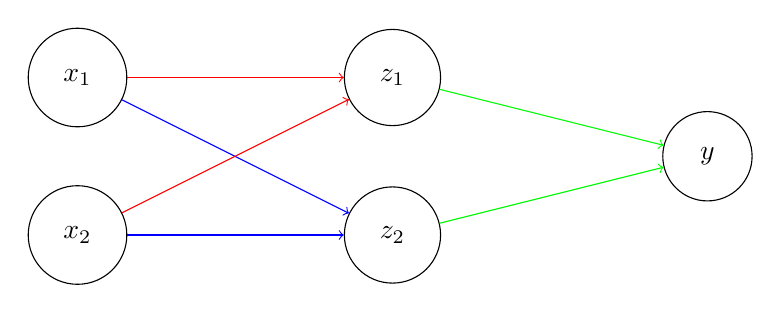
\begin{tikzpicture}
[   cnode/.style={draw=black,fill=#1,minimum width=3mm,circle},
]
\node[draw, circle, inner sep = 0.3cm] (A) at (0,1) {$x_1$};
\node[draw, circle, inner sep = 0.3cm] (B) at (0,-1) {$x_2$};
\node[draw, circle, inner sep = 0.3cm] (C) at (4,1) {$z_1$};
\node[draw, circle, inner sep = 0.3cm] (D) at (4,-1) {$z_2$};
\node[draw, circle, inner sep = 0.3cm] (E) at (8,0) {$y$};


\draw[->, red] (A) -- (C);
\draw[->, blue] (A) -- (D);
\draw[->, red] (B) -- (C);
\draw[->, blue] (B) -- (D);

\draw[->, green] (C) -- (E);
\draw[->, green] (D) -- (E);

\end{tikzpicture}

\end{center}


Para la neurona $z_1$ tenemos:
\[z_1=f(y_{\text{in}})=\left\{\begin{array}{lll}
1 & si & y_{\text{in}} \geq 1 \\
0 & si & y_{\text{in}} < 1
\end{array}\right. \text{ siendo } y_{\text{in}} = x_1+x_2\]

Para la neurona $z_2$ tenemos:
\[z_2=f(y_{\text{in}})=\left\{\begin{array}{lll}
1 & si & y_{\text{in}} \geq 2 \\
0 & si & y_{\text{in}} < 2
\end{array}\right. \text{ siendo } y_{\text{in}} = x_1+x_2\]

Por último, para la neurona $y$ tenemos:
\[y=f(y_{\text{in}})=\left\{\begin{array}{lll}
1 & si & y_{\text{in}} \geq 0 \\
0 & si & y_{\text{in}} < 0
\end{array}\right. \text{ siendo } y_{\text{in}} = z_1-z_2-1\]
\end{problem}

\begin{problem}[19]
Using the delta rule, find the weights required to perform the following classifications:
Vectors (1, 1, 1, 1) and (-1, 1, - 1, - 1) are members of the class (and therefore
have target value 1); vectors (1, 1, 1, - 1) and (1, - 1, - 1, 1) are not members of
the class (and have target value -1). Use a learning rate of .5 and starting weights
of 0. Using each of the training x vectors as input, test the response of the net.
\solution

La regla delta mencionada en el enunciado no es más que la regla de ajuste de pesos empleado en el proceso de aprendizaje de la red neuronal Adaline.

La siguiente tabla recoge los resultados obtenidos durante este proceso de aprendizaje
\small
\begin{center}
\begin{tabular}{|c|c|c|c|c|c|c|}
\hline
\textbf{Input} & \textbf{Pesos antes} &  \textbf{Bias antes} & \textbf{Out} & \textbf{Target} & \textbf{Pesos después} & \textbf{Bias después} \\
\hline
(1,1,1,1,1) & (0.00,0.00,0.00,0.00) & 0.00 & 1 & 1 & (0.50,0.50,0.50,0.50) & 0.50\\
(-1,1,-1,-1,1) & (0.50,0.50,0.50,0.50) & 0.50 & -1 & 1 & (-0.25,1.25,-0.25,-0.25) & 1.25\\
(1,1,1,-1,1) & (-0.25,1.25,-0.25,-0.25) & 1.25 & 1 & -1 & (-1.88,-0.38,-1.88,1.38) & -0.38\\
(1,-1,-1,1,1) & (-1.88,-0.38,-1.88,1.38) & -0.38 & 1 & -1 & (-3.06,0.81,-0.69,0.19) & -1.56\\
(1,1,1,1,1) & (-3.06,0.81,-0.69,0.19) & -1.56 & -1 & 1 & (-0.41,3.47,1.97,2.84) & 1.09\\
(-1,1,-1,-1,1) & (-0.41,3.47,1.97,2.84) & 1.09 & 1 & 1 & (-0.83,3.89,1.55,2.42) & 1.52\\
(1,1,1,-1,1) & (-0.83,3.89,1.55,2.42) & 1.52 & 1 & -1 & (-3.18,1.54,-0.80,4.77) & -0.84\\
(1,-1,-1,1,1) & (-3.18,1.54,-0.80,4.77) & -0.84 & 1 & -1 & (-3.69,2.05,-0.29,4.26) & -1.35\\
(1,1,1,1,1) & (-3.69,2.05,-0.29,4.26) & -1.35 & 1 & 1 & (-3.68,2.06,-0.28,4.27) & -1.34\\
\hline
\end{tabular}
\end{center}
\normalsize
\end{problem}

\section{Perceptrón multicapa}

\begin{center}
\includegraphics[width=0.8\textwidth]{img/figure6-12.png}
\end{center}

\begin{problem}[1]
Find the new weights when the net illustrated in Figure 6.12 is presented the input pattern (0, 1) and the target output is 1. Use a learning rate of $α = 0.25$, and the binary sigmoid activation function.

\solution

No hay más que seguir el algoritmo de entrenamiento para el perceptrón multicapa, descrito en el libro en las páginas 294, 295 y 296. En nuestro caso sólo tenemos un patrón de entrenamiento por lo que sólo deberemos realizar los pasos 3-8.

\begin{enumerate}
\item \textbf{Feedforward}
\begin{enumerate}
\item Asignamos a las neuronas de entrada los valores corresponientes al patrón dado:
\[x_1 = 0, \ x_2 = 1\]
\item Calculamos la salida de cada una de las neuronas de la capa intermedia:
\[\left\{ \begin{array}{l}
z_1 = f(0.4 -0.2) = f(0.2) = 0.55 \\
z_2 = f(0.6+0.3) =f(0.9) = 0.71
\end{array}\right.\]
\[\text{siendo }f(x) = \frac{1}{1+e^{-x}} \]

\item Calculamos el resultado para la neurona de salida
\[y_{in} = f(-0.3+0.5\cdot 0.55 + 0.1 \cdot 0.71)=f(0.046) = 0.51\]
\end{enumerate}
\item \textbf{Backpropagation of error}
\begin{enumerate}
\item Calculamos el valor δ de la neurona de salida
\[δ = (t-y_{in})f'(y_{in}) = (1-y_{in})f(y_{in})(1-f(y_{in})) = 0.12\]
Calculamos tambien la variación de peso que deberemos aplicar a las conexiones que llegan hasta esta neurona:
\[\left\{ \begin{array}{l}
Δw_1= αδz_1 = 0.017 \\
Δw_2= αδz_2 = 0.021 \\
Δw_0= αδ = 0.03
\end{array}\right.\]

\item Cada neurona oculta calcula su $δ_j$ como suma ponderada de los valores δ que llegan hasta ella, multiplicada por la derivada. En este caso:
\[\left\{ \begin{array}{l}
δ_1= ω_1 δ \cdot f'(z_1)= 0.06 \cdot 0.2475 = 0.015\\
δ_2= ω_2 δ \cdot f'(z_2)= 0.012 \cdot 0.205 = 0.0025
\end{array}\right.\]

Calculamos la variación de peso que deberemos aplicar a las conexiones que llegan hasta cada neurona:
\[\left\{ \begin{array}{l}
Δv_{11}= αδ_1x_1 = 0 \\
Δv_{21}= αδ_1x_2 = 0.00375 \\
Δv_{01}= αδ_1 = 0.00375 \\
Δv_{12}= αδ_2x_1 = 0 \\
Δv_{22}= αδ_2x_2 = 0.000625 \\
Δv_{02}= αδ_2 = 0.000625
\end{array}\right.\]
\end{enumerate}
\item \textbf{Update weights and biases}
\begin{enumerate}
\item Atendiendo a los incrementos calculados en los pasos anteriores tenemos los siguientes valores resultantes para los pesos:
\[\left\{ \begin{array}{l}
v_{11} = 0.7 \\
v_{21} = -0.1963 \\
v_{01} = 0.40375 \\
v_{12} = -0.4 \\
v_{22} = 0.300625 \\
v_{02} = 0.600625 \\
w_1    = 0.517 \\
w_2    = 0.221 \\
w_0    = - 0.27
\end{array}\right.\]
\end{enumerate}
\end{enumerate}
\end{problem}

\begin{problem}[2]
Find the new weights when the net illustrated in Figure 6.12 is presented the input pattern (-1, 1) and the target output is 1. Use a learning rate of $α = 0.25$, and the bipolar sigmoid activation function.

\solution

Repetimos los pasos del ejercicio anterior con diferentes valores de entrada. Cabe destacar que la función de activación empleada en esta ocasión es distinta al problema anterior.

\begin{enumerate}
\item \textbf{Feedforward}
\begin{enumerate}
\item Asignamos a las neuronas de entrada los valores corresponientes al patrón dado:
\[x_1 = -1, \ x_2 = 1\]
\item Calculamos la salida de cada una de las neuronas de la capa intermedia:
\[\left\{ \begin{array}{l}
z_1 = f(0.4 -0.2-0.7) = f(-0.5) = -0.25\\
z_2 = f(0.6+0.3+0.4) =f(1.3) = 0.57
\end{array}\right.\]
\[\text{siendo }f(x) = \frac{2}{1+e^{-x}} -1 \]

\item Calculamos el resultado para la neurona de salida
\[y_{in} = f(-0.3-0.5\cdot 0.25 + 0.1 \cdot 0.57)=f(-0.37) = -0.18\]
\end{enumerate}
\item \textbf{Backpropagation of error}
\begin{enumerate}
\item Calculamos el valor δ de la neurona de salida
\[δ = (t-y_{in})f'(y_{in}) = (1-y_{in})\frac{1}{2}(1+f(y_{in}))(1-f(y_{in})) = 0.57\]
Calculamos tambien la variación de peso que deberemos aplicar a las conexiones que llegan hasta esta neurona:
\[\left\{ \begin{array}{l}
Δw_1= αδz_1 = -0.036 \\
Δw_2= αδz_2 = 0.0812 \\
Δw_0= αδ = 0.1425
\end{array}\right.\]

\item Cada neurona oculta calcula su $δ_j$ como suma ponderada de los valores δ que llegan hasta ella, multiplicada por la derivada. En este caso:
\[\left\{ \begin{array}{l}
δ_1= ω_1 δ \cdot f'(z_1)= 0.13\\
δ_2= ω_2 δ \cdot f'(z_2)= 0.02
\end{array}\right.\]

Calculamos la variación de peso que deberemos aplicar a las conexiones que llegan hasta cada neurona:
\[\left\{ \begin{array}{l}
Δv_{11}= αδ_1x_1 = -0.0325 \\
Δv_{21}= αδ_1x_2 = 0.0325 \\
Δv_{01}= αδ_1 = 0.0325 \\
Δv_{12}= αδ_2x_1 = -0.005 \\
Δv_{22}= αδ_2x_2 = 0.005 \\
Δv_{02}= αδ_2 = 0.005
\end{array}\right.\]
\end{enumerate}
\item \textbf{Update weights and biases}
\begin{enumerate}
\item Atendiendo a los incrementos calculados en los pasos anteriores tenemos los siguientes valores resultantes para los pesos:
\[\left\{ \begin{array}{l}
v_{11}= αδ_1x_1 = 0.6675 \\
v_{21}= αδ_1x_2 = -0.1675 \\
v_{01}= αδ_1 = 0.4325 \\
v_{12}= αδ_2x_1 = -0.405 \\
v_{22}= αδ_2x_2 = 0.305 \\
v_{02}= αδ_2 = 0.605 \\
w_1    = 0.3575 \\
w_2    = 0.1812 \\
w_0    = -0.1575
\end{array}\right.\]
\end{enumerate}
\end{enumerate}

\end{problem}

\begin{problem}[3]
Find the new weights when the net illustrated in Figure 6.12 is presented the input pattern (0, 1) and the target output is 0.8. Use a learning rate of $α = 0.25$, and the binary sigmoid activation function.

\solution

En esta ocasión estamos ante una modificación del ejercicio 1 de esta sección en el que ha cambiado el valor esperado de la neurona.

\begin{enumerate}
\item \textbf{Feedforward}
\begin{enumerate}
\item Asignamos a las neuronas de entrada los valores corresponientes al patrón dado:
\[x_1 = 0, \ x_2 = 1\]
\item Calculamos la salida de cada una de las neuronas de la capa intermedia:
\[\left\{ \begin{array}{l}
z_1 = f(0.4 -0.2) = f(0.2) = 0.55 \\
z_2 = f(0.6+0.3) =f(0.9) = 0.71
\end{array}\right.\]
\[\text{siendo }f(x) = \frac{1}{1+e^{-x}} \]

\item Calculamos el resultado para la neurona de salida
\[y_{in} = f(-0.3+0.5\cdot 0.55 + 0.1 \cdot 0.71)=f(0.046) = 0.51\]
\end{enumerate}
\item \textbf{Backpropagation of error}
\begin{enumerate}
\item Calculamos el valor δ de la neurona de salida
\[δ = (t-y_{in})y_{in}(1-y_{in}) = 0.0725\]
Calculamos tambien la variación de peso que deberemos aplicar a las conexiones que llegan hasta esta neurona:
\[\left\{ \begin{array}{l}
Δw_1= αδz_1 = 0.00997 \\
Δw_2= αδz_2 = 0.0129 \\
Δw_0= αδ    = 0.0181
\end{array}\right.\]

\item Cada neurona oculta calcula su $δ_j$ como suma ponderada de los valores δ que llegan hasta ella, multiplicada por la derivada. En este caso:
\[\left\{ \begin{array}{l}
δ_1= ω_1 δ \cdot z_1(1-z_1)= 0.0363 \cdot 0.2475 = 0.00898\\
δ_2= ω_2 δ \cdot z_2(1-z_2)= 0.00725 \cdot 0.205 = 0.00149
\end{array}\right.\]

Calculamos la variación de peso que deberemos aplicar a las conexiones que llegan hasta cada neurona:
\[\left\{ \begin{array}{l}
Δv_{11}= αδ_1x_1 = 0 \\
Δv_{21}= αδ_1x_2 = 0.00225 \\
Δv_{01}= αδ_1    = 0.00225 \\
Δv_{12}= αδ_2x_1 = 0 \\
Δv_{22}= αδ_2x_2 = 0.000373 \\
Δv_{02}= αδ_2    = 0.000373
\end{array}\right.\]
\end{enumerate}
\item \textbf{Update weights and biases}
\begin{enumerate}
\item Atendiendo a los incrementos calculados en los pasos anteriores tenemos los siguientes valores resultantes para los pesos:
\[\left\{ \begin{array}{l}
v_{11} = 0.7 \\
v_{21} = -0.19775 \\
v_{01} = 0.40225 \\
v_{12} = -0.4 \\
v_{22} = 0.300373 \\
v_{02} = 0.600373 \\
w_1    = 0.50997 \\
w_2    = 0.1129 \\
w_0    = - 0.2819
\end{array}\right.\]
\end{enumerate}
\end{enumerate}
\end{problem}



\begin{problem}[4]
Find the new weights when the net illustrated in Figure 6.12 is presented the input pattern (-1, 1) and the target output is 0.8. Use a learning rate of $α = 0.25$, and the bipolar sigmoid activation function.

\solution

Repetimos los pasos del ejercicio 2 con diferente valor de salida.

\begin{enumerate}
\item \textbf{Feedforward}
\begin{enumerate}
\item Asignamos a las neuronas de entrada los valores corresponientes al patrón dado:
\[x_1 = -1, \ x_2 = 1\]
\item Calculamos la salida de cada una de las neuronas de la capa intermedia:
\[\left\{ \begin{array}{l}
z_1 = f(0.4 -0.2-0.7) = f(-0.5) = -0.25\\
z_2 = f(0.6+0.3+0.4) =f(1.3) = 0.57
\end{array}\right.\]
\[\text{siendo }f(x) = \frac{2}{1+e^{-x}} -1 \]

\item Calculamos el resultado para la neurona de salida
\[y_{in} = f(-0.3-0.5\cdot 0.25 + 0.1 \cdot 0.57)=f(-0.37) = -0.18\]
\end{enumerate}
\item \textbf{Backpropagation of error}
\begin{enumerate}
\item Calculamos el valor δ de la neurona de salida
\[δ = (t-y_{in})f'(y_{in}) = (1-y_{in})\frac{1}{2}(1+f(y_{in}))(1-f(y_{in})) = 0.47\]
Calculamos tambien la variación de peso que deberemos aplicar a las conexiones que llegan hasta esta neurona:
\[\left\{ \begin{array}{l}
Δw_1= αδz_1 = -0.029 \\
Δw_2= αδz_2 = 0.0678 \\
Δw_0= αδ = 0.1186
\end{array}\right.\]

\item Cada neurona oculta calcula su $δ_j$ como suma ponderada de los valores δ que llegan hasta ella, multiplicada por la derivada. En este caso:
\[\left\{ \begin{array}{l}
δ_1= ω_1 δ \cdot f'(z_1)= 0.111\\
δ_2= ω_2 δ \cdot f'(z_2)= 0.0159
\end{array}\right.\]

Calculamos la variación de peso que deberemos aplicar a las conexiones que llegan hasta cada neurona:
\[\left\{ \begin{array}{l}
Δv_{11}= αδ_1x_1 = -0.0278 \\
Δv_{21}= αδ_1x_2 = 0.02786 \\
Δv_{01}= αδ_1    = 0.02786 \\
Δv_{12}= αδ_2x_1 = -0.0039 \\
Δv_{22}= αδ_2x_2 = 0.00399 \\
Δv_{02}= αδ_2    = 0.00399
\end{array}\right.\]

\end{enumerate}
\item \textbf{Update weights and biases}
\begin{enumerate}
\item Atendiendo a los incrementos calculados en los pasos anteriores tenemos los siguientes valores resultantes para los pesos:
\[\left\{ \begin{array}{l}
v_{11} =  0.672133\\
v_{21} =  -0.17213\\
v_{01} =  0.427866\\
v_{12} =  -0.40399\\
v_{22} =  0.303991\\
v_{02} =  0.603991\\
w_0     =  -0.18141\\
w_1     =  0.470957\\
w_2     =  0.167788
\end{array}\right.\]
\end{enumerate}
\end{enumerate}

\end{problem}

\begin{problem}[5]
Repeat Exercises 6.1-6.4 using a slope parameter of $σ = 3.0$. Does this increase, or decrease the amount of learning (size of the weight changes)?

\solution

La siguiente tabla recoje los resultados obtenidos al realizar el cambio indicado sobre los ejercicios anteriores y comparar la cantidad de aprendizaje.

\begin{center}
\begin{tabular}{|c|c|c|}
\hline
\textbf{Ejercicio} & \textbf{Aprendizaje con σ=1} & \textbf{Aprendizaje con σ=3} \\
\hline
1 & 0.0414 & 0.1196\\
2 & 0.1781 & 0.6072\\
3 & 0.0244 & 0.0618\\
4 & 0.1479 & 0.5337\\
\hline
\end{tabular}
\end{center}

Podemos obsevar que la cantidad de aprendizaje ha aumentado considerablemente.

Este incremento es bastante lógico si nos percatamos de que el cambio realizado en la función $f(x)$ implica un cambio de la derivada que ahora pasa a ser tres veces lo que era antes.

Puesto que el aprendizaje depende del valor de la derivada, al triplicar este valor estamos aumentando la cantidad de aprendizaje por patrón.
\end{problem}

\begin{center}
\includegraphics[width=0.8\textwidth]{img/figure6-12.png}
\end{center}

\begin{problem}[6]
A neural network is being trained on the data for XOR problem. The architecture and the values of the weights and biases are shown in Figure 6.13.

\ppart Using the binary sigmoid, compute the activations for each of the units when the input vector (0, 1) is presented. Find the delta factors for the output and hidden units. Using a learning rate of $α = 0.25$, compute the weight corrections. Find the new weights (and biases).
\ppart Repeat for the input vector (1, 0).
\ppart Interpret the differences between the weight changes on the connection to the output unit and the weight changes to the hidden units in parts a and b.
\solution

\spart

Una vez más, llevamos a cabo los pasos correspondientes del proceso de entrenamiento del perceptrón multicapa.

\begin{enumerate}
\item \textbf{Feedforward}
\begin{enumerate}
\item Asignamos a las neuronas de entrada los valores corresponientes al patrón dado:
\[x_1 = 0, \ x_2 = 1\]
\item Calculamos la salida de cada una de las neuronas de la capa intermedia:
\[\left\{ \begin{array}{l}
z_1 = f(2+9.2) = f(11.2) = 0.999\\
z_2 = f(8.8-0.1) =f(8.7) = 0.999
\end{array}\right.\]
\[\text{siendo }f(x) = \frac{1}{1+e^{-x}}\]

\item Calculamos el resultado para la neurona de salida
\[y_{in} = f(-0.8-4.5\cdot 0.999 + 5.3 \cdot 0.999)=f(-0.0008) = 0.4999\]
\end{enumerate}
\item \textbf{Backpropagation of error}
\begin{enumerate}
\item Calculamos el valor δ de la neurona de salida
\[δ = (t-y_{in})f'(y_{in}) = (1-y_{in})f(y_{in})(1-f(y_{in})) = 0.125\]
Calculamos tambien la variación de peso que deberemos aplicar a las conexiones que llegan hasta esta neurona:
\[\left\{ \begin{array}{l}
Δw_1= αδz_1 = 0.03126 \\
Δw_2= αδz_2 = 0.03126 \\
Δw_0= αδ = 0.03126
\end{array}\right.\]

\item Cada neurona oculta calcula su $δ_j$ como suma ponderada de los valores δ que llegan hasta ella, multiplicada por la derivada. En este caso:
\[\left\{ \begin{array}{l}
δ_1= ω_1 δ \cdot f'(z_1)= -7.695\\
δ_2= ω_2 δ \cdot f'(z_2)= 0.000110
\end{array}\right.\]

Calculamos la variación de peso que deberemos aplicar a las conexiones que llegan hasta cada neurona:
\[\left\{ \begin{array}{l}
Δv_{11}= αδ_1x_1 = 0.000001924\\
Δv_{21}= αδ_1x_2 = -0.0\\
Δv_{01}= αδ_1    = -0.00000192\\
Δv_{12}= αδ_2x_1 = 0.0\\
Δv_{22}= αδ_2x_2 = 0.000027593\\
Δv_{02}= αδ_2    = 0.000027593
\end{array}\right.\]


\end{enumerate}
\item \textbf{Update weights and biases}
\begin{enumerate}
\item Atendiendo a los incrementos calculados en los pasos anteriores tenemos los siguientes valores resultantes para los pesos:
\[\left\{ \begin{array}{l}
v_{11} =    -2.0\\
v_{21} =    9.19999807633\\
v_{01} =    1.99999807633\\
v_{12} =    4.3\\
v_{22} =    8.80002759291\\
v_{02} =    -0.0999724070945\\
w_0     =  -0.768737173636\\
w_1     =  -4.46873760112\\
w_2     =  5.33125761929
\end{array}\right.\]

\end{enumerate}
\end{enumerate}

\spart

Tomando ahora el vector de entrada $(1,0)$ obtenemos:

\begin{enumerate}
\item \textbf{Feedforward}
\begin{enumerate}
\item Asignamos a las neuronas de entrada los valores corresponientes al patrón dado:
\[x_1 = 1, \ x_2 = 0\]
\item Calculamos la salida de cada una de las neuronas de la capa intermedia:
\[\left\{ \begin{array}{l}
z_1 = f(2-2) = f(0) = 0.5\\
z_2 = f(4.3-0.1) =f(4.2) = 0.985
\end{array}\right.\]
\[\text{siendo }f(x) = \frac{1}{1+e^{-x}}\]

\item Calculamos el resultado para la neurona de salida
\[y_{in} = f(-0.8-4.5\cdot 0.5 + 5.3 \cdot 0.985)=f(2.17) = 0.8977\]
\end{enumerate}
\item \textbf{Backpropagation of error}
\begin{enumerate}
\item Calculamos el valor δ de la neurona de salida
\[δ = (t-y_{in})f'(y_{in}) = (1-y_{in})f(y_{in})(1-f(y_{in})) = -0.0094\]
Calculamos tambien la variación de peso que deberemos aplicar a las conexiones que llegan hasta esta neurona:
\[\left\{ \begin{array}{l}
Δw_1= αδz_1 = 0.00117 \\
Δw_2= αδz_2 = 0.00231 \\
Δw_0= αδ = 0.002349
\end{array}\right.\]

\item Cada neurona oculta calcula su $δ_j$ como suma ponderada de los valores δ que llegan hasta ella, multiplicada por la derivada. En este caso:
\[\left\{ \begin{array}{l}
δ_1= ω_1 δ \cdot f'(z_1)= -0.0106\\
δ_2= ω_2 δ \cdot f'(z_2)= 0.000725
\end{array}\right.\]

Calculamos la variación de peso que deberemos aplicar a las conexiones que llegan hasta cada neurona:
\[\left\{ \begin{array}{l}
Δv_{11}= αδ_1x_1 = -0.0026432\\\
Δv_{21}= αδ_1x_2 = -0.0\\
Δv_{01}= αδ_1    = -0.0026433\\
Δv_{12}= αδ_2x_1 = 0.00018126\\
Δv_{22}= αδ_2x_2 = 0.0\\
Δv_{02}= αδ_2    = 0.00018126
\end{array}\right.\]

\end{enumerate}
\item \textbf{Update weights and biases}
\begin{enumerate}
\item Atendiendo a los incrementos calculados en los pasos anteriores tenemos los siguientes valores resultantes para los pesos:
\[\left\{ \begin{array}{l}
v_{11} =   -2.00264327978 \\
v_{21} =   9.2 \\
v_{01} =   1.99735672022 \\
v_{12} =   4.30018125974 \\
v_{22} =   8.8 \\
v_{02} =   -0.0998187402577 \\
w_0     = -0.79765041797 \\
w_1     = -4.49882520898 \\
w_2     = 5.30231486923
\end{array}\right.\]
\end{enumerate}
\end{enumerate}

\spart

\end{problem}

\begin{center}
\includegraphics[width=0.8\textwidth]{img/figure6-13.png}
\end{center}

\begin{problem}[7]
Explore the role of the weights in backpropagation training by finding weights that are reasonable in size, but for which very little learning will occur. For example, in Exercise 1 of this section, if $v_{02}+v_{22}\approx 0$, then $z_2 \approx 0$ so that $Δw_{21}\approx 0$, even if an error occurs at the output unit. Are there combinations of other weights for which very little
learning will occur? Consider the situation for Exercise 2 of this section..

\solution

En general siempre que ajustemos los pesos de forma que una neurona de la capa intermedia tenga salida valor de activación 0, estamos haciendo que no se produzca nada de aprendizaje en la conexión que lleva de esa neurona a la neurona de salida.

Otra situación en la que se produce muy poco aprendizaje es el momento en el que el valor δ es 0. Esto ocurre cuando la derivada de la función toma valor 0, cosa que ocurre cuando $f(x)\approx 1$.
\end{problem}

\section{Resumen de contenidos Teóricos}
Hasta ahora hemos trabajado con dos tipos de redes neuronales diferentes: aquellas que sólo tienen dos capas de neuronas (la de entrada y la de salida) y las redes con una capa intermedia.

Todas las redes funcionan de la misma manera: los valores se predicen atendiendo a las funciones de activación; para cada neurona distinta de las neuronas de entrada tenemos un bias, que actúa como una entrada con valor 1 permanente; y cada red tiene un algoritmo de aprendizaje que nos permite ajustar los pesos adecuadamente.

\subsection{Algoritmos de aprendizaje}
\subsubsection{Red Hebb}
\begin{enumerate}
\item Inicializamos los pesos a 0.
\item Para cada patrón de entrenamiento:
\begin{enumerate}
\item Tomamos la salida esperada $t$
\item Ajustamos los pesos según la regla:
\[w_i = w_i + x_i\cdot t\]
\[b = b + t\]
\end{enumerate}
\end{enumerate}

\subsubsection{Perceptrón}
\begin{enumerate}
\item Inicializamos los pesos a 0.
\item Definimos un factor de aprendizaje α
\item Mientras no se cumpla la condición de parada:
\begin{enumerate}
\item Para cada patrón de entrenamiento
\begin{enumerate}
\item Hacemos trabajar a la red sobre el patrón obteniendo
\[y\_in = b + \sum_i x_i\cdot w_i\]
\[y = \left\{ \begin{array}{lll}
1 & \text{si} & y\_in > \theta \\
0 & \text{si} & -\theta \geq  y\_in \geq  \theta \\
-1 & \text{si} & y\_in < -\theta
\end{array}\right.\]

\item Si el resultado predicho no coincide con el esperado, es decir si $y\neq t$ actualizamos los pesos según la regla
\[w_i = w_i + αtx_i\]
\[b = b + αt\]
\end{enumerate}
\item Condición de parada: Si ningún peso ha cambiado paramos.
\end{enumerate}
\end{enumerate}

\subsubsection{Adaline}
La regla de aprendizaje de esta red neuronal se apoya en la idea de \textbf{minimizar el error cuadrático medio}. Veamos cómo funciona esta regla:
\begin{enumerate}
\item Inicializamos los pesos con valores aleatorios.
\item Definimos un factor de aprendizaje α
\item Mientras no se cumpla la condición de parada:
\begin{enumerate}
\item Para cada patrón de entrenamiento
\begin{enumerate}
\item Hacemos trabajar a la red sobre el patrón obteniendo
\[y\_in = b + \sum_i x_i\cdot w_i\]

\item Actualizamos los pesos
\[w_i = w_i + α(t-y\_in)x_i\]
\[b = b + αt\]
\end{enumerate}
\item Condición de parada: Si el mayor cambio aplicado a los pesos es menor que un cierto valor indicado previamente, paramos.
\end{enumerate}
\end{enumerate}

El \concept{error cuadrático medio} viene dado por la ecuación
\[E = \sum_{j=1}^m(t_j-y\_in_j)^2\]

siendo $E$ una función que (fijando una entrada) depende de todos los pesos de la red. Si queremos calcular los pesos que minimizan el error cuadrático medio para esa entrada lo que debemos hacer es modificar los pesos en la dirección del gradiente. El \concept{gradiente} de una superficie es un vector que nos da la dirección de máximo crecimiento (consecuentemente, su opuesto nos da la dirección de máximo decrecimiento).

Para obtener el vector gradiente lo que único que debemos hacer es derivar respecto a cada coordenada. Vamos a ello:

\[\frac{\partial E}{\partial w_{ij}} = \frac{\partial}{\partial w_{ij}}\sum_{k=1}^m(t_k-y\_in_k)^2 = \frac{\partial}{\partial w_{ij}} (t_j - y\_in_j)^2 = -2(t_j-y\_in_j)\frac{\partial}{\partial w_{ij}}y\_in_j\]
Sabiendo que
\[y\_in_j = \sum_{i=1}^n x_i w_{ij}\]
tenemos
\[\frac{\partial E}{\partial w_ij}=-2(t_j-y\_in_j)x_i\]

Podemos observar que, en cada peso, la variación aplicada por el algoritmo de aprendizaje es el opuesto de este valor.


\subsubsection{Perceptrón multicapa}
\begin{enumerate}
\item Inicializamos los pesos con valores aleatorios.
\item Definimos un factor de aprendizaje α
\item Mientras no se cumpla la condición de parada:
\begin{enumerate}
\item \textbf{Feedforward}
\begin{enumerate}
\item Asignamos a las neuronas de entrada los valores corresponientes al patrón dado
\item Calculamos la salida de cada una de las neuronas de la capa intermedia, así como su entrada neta
\[z\_in_j = v_{0j} + \sum_{i=1}^nx_iv_{ij}\]
\[z_j=f(z\_in_j)\]
\item Calculamos la salida de cada neurona de salida, así como su entrada neta
\[y\_in_k = w_{0k} + \sum_{j=1}^pz_jw_{jk}\]
\[y_k = f(y\_in_k)\]
\end{enumerate}
\item \textbf{Backpropagation of error}
\begin{enumerate}
\item Calculamos el valor δ de cada neurona de salida
\[δ_k = (t-y_k)f'(y\_in_k) \]
Calculamos tambien la variación de peso que deberemos aplicar a las conexiones que llegan hasta esta neurona:
\[Δw_{jk}= αδ_kz_j\]
\[Δw_{0k}= αδ_k\]

\item Cada neurona oculta calcula su $δ\_in_j$ como suma ponderada de los valores δ que llegan hasta ella, multiplicada por la derivada.
\[δ\_in_j = \sum_{k=1}^m δ_kw_{jk}\]
\[δ_j= δ\_in_j \cdot f'(z\_in_j)\]

Calculamos la variación de peso que deberemos aplicar a las conexiones que llegan hasta cada neurona:
\[Δv_{ij} = αδ_jx_i\]
\[Δv_{0j} = αδ_j\]

\end{enumerate}
\item \textbf{Update weights and biases}
\begin{enumerate}
\item Atendiendo a los incrementos calculados en los pasos anteriores actualizamos los pesos
\end{enumerate}
\end{enumerate}
\item Comprobamos la condición de parada, que no viene definida por defecto.
\end{enumerate}

Para la única red multicapa que hemos estudiado hasta el momento hay una diferencia más, aparte de la existencia de una capa intermedia de neuronas. Para el \textbf{perceptrón multicapa} las neuronas intermedias y la de salida tienen función de activación continua con lo que el valor emitido puede ser cualquiera dentro de un intervalo.

Para un percpetrón multicapa con salida binaria la función de activación suele ser
\[f(x) = \frac{1}{1+e^{-x}}, \text{ conocida como sigmoidal binaria}\]
mientras que si la salida es bipolar suele tomarse la función de activación de la forma
\[f(x) = \frac{2}{1+e^{-x}}+1, \text{ conocida como sigmoidal bipolar}\]

En general es necesario emplear funciones continuas cuyo recorrido varíe desde 0 hasta 1, en el caso de salida binaria, o desde -1 hasta 1, para el caso de salida bipolar.

En concreto se emplean funciones como las mencionadas anteriormente puesto que su derivada evaluada en un punto $x_0$ puede calcularse cómodamente a partir de la evaluación de la función en ese mismo punto. Así, a la hora de calcular $f'(z\_in_j)$ no tenemos que realizar ninguna evaluación de función, ya que $f(z\_in_j)$ ya se calculó previamente. La importancia de este detalle radica en el hecho de que evaluar funciones es uno de los procesos más costosos (y por tanto más lentos) que puede realizar un ordenador, por lo que conviene evitarlos. Así tenemos
\[f'(x) = f(x) (1-f(x)), \text{ para la sigmoidal binaria}\]
y
\[f'(x) = \frac{1}{2}(1+f(x))(1-f(x)), \text{ para la sigmoidal bipolar}\]

Aunque pueden emplearse redes neuronales multicapa con más de una capa intermedia, por lo general, con una sola capa intermedia es suficiente para enseñar a la red a resolver cualquier tipo de problema.

\subsection{Sobreaprendizaje}

El objetivo de las redes neuronales es ser capaz de predecir la salida de ciertos patrones y para ello se les entrena con unos patrones dados de los que conocemos su salida.

No obstante, si entrenamos demasiado a la red, puede que esta se vuelve muy especifica para los patrones de entrenamiento dados\footnote{Esto no ocurre con el perceptrón, que sólo actualiza pesos si predice mal la salida} de modo que cuando analice otros datos parecidos a los iniciales no sea capaz de notarlo.

Es por ello que hay que encontrar un punto justo entre precisión clasificando los patrones de entrenamiento y capacidad de aceptar variaciones pequeñas, manteniendo una correcta clasificación.

Esto nos lleva a que (en las redes multicapa) podamos cambiar el algoritmo de entrenamiento considerando que en cada iteración, en lugar de movernos en la dirección del gradiente para la entrada dada, nos movemos en la dirección combinación del gradiente actual y el de la entrada anterior. Esto nos permite no ser demasiado específicos.

Este entrenamiento es conocido como el método del \textbf{momento}. En esta ocasión la actualización de los pesos se lleva a cabo mediante las fórmulas:
\[Δw_{jk}(t+1) = αδ_kz_j + μΔw_{jk}(t)\]
y
\[Δv_{ij}(t+1) = αδ_jx_i + μΔv_{ij}(t)\]
lo que implica la necesidad de recordar los pesos de la iteración anterior.

\subsection{Modificaciones en la función de activación}
\subsubsection{Cambiando el recorrido}
En ocasiones puede interesarnos que el recorrido de la función de activación $f(x)$ oscile entre $a$ y $b$ en lugar de entre $0$ y $1$. Para conseguirlo basta con tomar la función
\[g(x)=αf(x)-β, \text{ siendo } α=b-a \text{ y } β = -a\]

Al hacer este cambio seguimos conservando la propiedad de que la derivada puede evaluarse a partir de la evaluación de la función en el punto pues:
\[g'(x) = \frac{1}{α}(β+g(x))(α-β-g(x))\]

En concreto si queremos que $a=-1$ y $b=1$, es decir, queremos la función sigmoidal bipolar, este procedimiento nos permite obtener el resultado visto anteriormente.

\subsubsection{Cambiando la pendiente}
En ocasiones puede interesarnos cambiar la pendiente de la funció de activación de modo que el paso del valor más bajo al más alto posible sea más rápido.

Esto implica considerar la función sigmoidal binaria como:
\[f(x) = \frac{1}{1+e^{-σx}}\]
donde $σ=1$ para los casos vistos hasta ahora. Cuanto mayor sea el valor σ más brusco será el crecimiento de la función, como muestra la figura \ref{fig:sigmoidalCambioSigma}

\begin{figure}[hbtp]
\centering
\includegraphics[width = 0.6\textwidth]{img/sigmoidalCambioSigma.png}
\caption{Función sigmoidal para $σ=1$ (línea continua) y $σ=3$ (línea discontinua)}
\label{fig:sigmoidalCambioSigma}
\end{figure}

En esta ocasión seguimos conservando la buena propiedad comentada anteriormente respecto a la evaluación de la derivada, teniendo
\[f'(x) = σf(x)(1-f(x))\]

\section{Asociación de patrones}
\subsection{Regla Hebb}

\begin{problem}[1]\label{ej:3_1}
Show that yet another way of viewing the formation of the weight matrix for Hebb learning is to form an $n\times p$ matrix $S$ whose columns are the input paterns
\[s(p) = (s_1(p),\cdots, s_i(p),\cdots s_n(p))\]
es decir
\[S = \left( \begin{array}{ccccc}
s_1(1) & . & . & . & s_1(P) \\
. & . & . & . & . \\
s_i(1) & . & . & . & s_i(P) \\
. & . & . & . & . \\
s_n(1) & . & . & . & s_n(P) \\
\end{array}\right)\]

and a $p \times m$ matrix $T$ whose rows are the output patterns
\[t(p) = (t_1(p)), \cdots, t_j(p), \cdots t_m(p))\]
es decir
\[T = \left( \begin{array}{ccccc}
t_1(1) & . & . & . & t_m(p) \\
. & . & . & . & . \\
. & . & . & . & . \\
. & . & . & . & . \\
t_1(1) & . & . & . & t_m(p) \\
\end{array}\right)\]

then the product $S\cdot T$ gives the weight matrix $W$:
\[W = S\cdot T =  \left( \begin{array}{ccccc}
\sum_{p=1}^P s_1(p)t_1(p) & . & . & . & \sum_{p=1}^P s_1(p)t_m(p) \\
. & . & . & . & . \\
. & . & . & . & . \\
. & . & . & . & . \\
\sum_{p=1}^P s_n(p)t_1(p) & . & . & . & \sum_{p=1}^P s_n(p)t_m(p) \\
\end{array}\right)\]
\solution

\doneby{Pedro}

La regla de aprendizaje Hebb consiste en actualizar los pesos en cada iteración según la fórmula
\[Δω_{ij} = x_iy_j\]
con independencia de si la predicción fue correcta o no.

Tras repetir este proceso de aprendizaje con todos los patrones tendremos:
\[Δω_{ij} = \sum_{x:y} x_iy_j\]
que es lo mismo que obtenemos multiplicando las matrices $S$ y $T$ descritas en el enunciado.

\end{problem}

\begin{problem}[2]
Show the computations for the first component of the response of a Hebb net for an input vector and how this response depends on whether the input vector is orthogonal to the other vectors stored in the net.
\solution

\doneby{Pedro}

Partiendo de la matriz $W$ calculda en el ejercicio anterior, tomando ahora un vector cualquiera $\vx = (s_1(x),\ldots, s_n(x))$ al calcular la primera componente del vector de salida tendríamos:

\begin{equation}\label{eq:salida}
\vx \cdot W[1:] = s(x) \cdot \sum_{p=1}^Ps(p)^Tt_1(p) = \sum_{p=1}^Ts(x)\cdot s(p)^Tt_1(p)
\end{equation}

Los patrones ``almacenados'' en la red son simplemente los patrones usados para entrenamiento, para los que la red se ha preparado para dar una respuesta ``perfecta''.

Si el vector de entrada que estamos analizando en este momento $\vx$ es perpendicular a alguno de los vectores usados para el entrenamiento tendremos
\[s(x)\cdot s^T(p) = 0\]

con lo que ciertos términos del sumatorio \ref{eq:salida} desaparecerían (al hacerse nulos)

\end{problem}

\subsection{Red neuronal heteroasociativa}

\begin{problem}[3]
Find the weight matrix for Example 3.1 using the results of Exercise \ref{ej:3_1}.
\solution

\doneby{Pedro}

El ejemplo 3.1 nos plantea una red neuronal para la que nos da unos patrones de entrenamiento. Disponiendo la información de estos patrones en forma de matriz tenemos:

\[S = \left( \begin{array}{cccc}
1 & 1 & 0 & 0\\
0 & 1 & 0 & 0\\
0 & 0 & 0 & 1\\
0 & 0 & 1 & 1
\end{array}\right), \ \ T = \left( \begin{array}{cc}
1 & 0 \\
1 & 0 \\
0 & 1 \\
0 & 1
\end{array}\right)\]

Atendiendo al ejercicio \ref{ej:3_1} lo único que debemos hacer es multiplicar estas dos matrices, con lo que obtenemos la matriz de pesos:
\[W = S\cdot T = \left( \begin{array}{cc}
2 & 0 \\
1 & 0 \\
0 & 1 \\
0 & 2
\end{array}\right)\]

\end{problem}

\begin{problem}[4]
Test Example 3.6 on the input training vectors. Then test on input vectors that are
similar to the input training vectors.
\solution

\doneby{Pedro}

En el ejemplo 3.6 se calcula la matriz de pesos correspondiende a los patrones de entrenamiento dados obteniendo:
\[W = \left( \begin{array}{cc}
4 & -4 \\
2 & -2 \\
-2 & 2 \\
-4 & 4
\end{array}\right)\]

Puesto que las salidas son binarias, sabemos que la función de activación es:
\[f(x) = \left\{ \begin{array}{lll} 1 & si & x>0 \\ 0 & si & x\leq 0 \end{array}\right. \]

La siguiente tabla recoge los resultados obtenidos al clasificar los patrones de entrenamiento (4 primeras filas) y pequeñas modificaciones de los mismos:

\begin{center}
\begin{tabular}{|c|c|c|}
\hline
\textbf{Entrada } & \textbf{Salida esperada} & \textbf{Salida predicha} \\
\hline
(1,0,0,0) & (1,0) & (1,0) \\
(1,1,0,0) & (1,0) & (1,0) \\
(0,0,0,1) & (0,1) & (0,1) \\
(0,0,1,1) & (0,1) & (0,1) \\
(1,0,1,0) & (1,0) & (1,0) \\
(1,1,0,1) & (1,0) & (1,0) \\
(1,0,0,1) & ? & (0,0) \\
(1,0,1,1) & (0,1) & (0,1) \\
\hline
\end{tabular}
\end{center}
\end{problem}

\begin{problem}[5]
Test Example 3.7 using the training input vectors. Then test with input vectors that
are the training vector with one ``mistake''.
\solution
\doneby{Pedro}

Tenemos la misma matriz de pesos del paso anterior pero en esta ocasión la salida es bipolar, por lo que estamos empleando una función de activación diferente:
\[f(x) = \left\{ \begin{array}{lll} 1 & si & x>0 \\ 0 & si & x=0 \\ -1 & si & x< 0 \end{array}\right. \]

Con las mismas entradas empleadas en el ejercicio anterior obtenemos:
\begin{center}
\begin{tabular}{|c|c|c|}
\hline
\textbf{Entrada } & \textbf{Salida esperada} & \textbf{Salida predicha} \\
\hline
(1,-1,-1,-1) & (1,-1) & (1,-1) \\
(1,1,-1,-1)  & (1,-1) & (1,-1) \\
(-1,-1,-1,1) & (-1,1) & (-1,1) \\
(-1,-1,1,1)  & (-1,1) & (-1,1) \\
(1,-1,1,-1)  & (1,-1) & (1,-1) \\
(1,1,-1,1)   & (1,-1) & (1,-1) \\
(1,-1,-1,1)  & ?      & (0,0)  \\
(1,-1,1,1)   & (-1,1) & (-1,1) \\
\hline
\end{tabular}
\end{center}

No se observa ningún cambio en esta situación. No obstante, podría ocurrir que en lugar de producirse \emph{errores} en el patrón de entrada simplemente tengamos \emph{faltas de información}. En este caso tendríamos:
\begin{center}
\begin{tabular}{|c|c|c|}
\hline
\textbf{Entrada } & \textbf{Salida esperada} & \textbf{Salida predicha} \\
\hline
(1,0,-1,-1) & (1,-1)  & (1,-1) \\
(0,1,-1,-1)  & (1,-1) & (1,-1) \\
(-1,0,-1,1) & (-1,1)  & (-1,1) \\
(0,-1,1,1)  & (-1,1)  & (-1,1) \\
\hline
\end{tabular}
\end{center}
\end{problem}

\begin{problem}[6]
\ppart Use the hybrid (binary/bipolar) form of Hebb rule learning as described in Example
3.6 to find the weight matrix for the associative memory network based on the
following binary input-output vector pairs:

\[\begin{array}{cc}
s(1) = (1,0,0,0) & t(1)=(1,0)\\
s(2) = (1,0,0,1) & t(2) = (1,0)\\
s(3)=(0,1,0,0) & t(3) = (0,1) \\
s(4) = (0,1,1,0) & t(4) = (0,1)
\end{array}\]

\ppart  Using the unit step function (with threshold 0) as the output units' activation function, test the response of your network on each of the input patterns. Describe the results obtained.

\ppart Test the response of your network on various combinations of input patterns with``mistakes'' or ``missing data'' (as in Example 3.8). Discuss the results you observe.

\solution

\doneby{Pedro}

\spart

Emplear la forma híbrida simplemente consiste en tomar los vectores de entrenamiento en forma binaria pero \emph{considerarlos bipolares} a la hora del entrenamiento.

Como los estamos considerando binarios, la función de activación que trabajará en la red será la correspondiente a datos binarios, aunque haya sido entrenada de forma bipolar (de ahí que se llamen hibridas).

La forma de realizar esto consiste en sustituir la fórmula del peso de cada conexión del algoritmo Hebb:
\[w_{ij} = \sum_p s_i(p)t_j(p)\]
por
\[w_{ij} = \sum_p (2\cdot s_i(p)-1) \cdot (2\cdot t_j(p)-1)\]

Usando los datos de entrenamiento:
\[\begin{array}{cc}
s(1) = (1,0,0,0) & t(1) = (1,0)\\
s(2) = (1,0,0,1) & t(2) = (1,0)\\
s(3)=  (0,1,0,0) & t(3) = (0,1) \\
s(4) = (0,1,1,0) & t(4) = (0,1)
\end{array}\]

tenemos
\[W = S\cdot T = \left( \begin{array}{cc}
4 & -4 \\
-4 & 4 \\
-2 & 2 \\
2 & -2
\end{array}\right)\]

\spart

\begin{center}
\begin{tabular}{|c|c|c|}
\hline
\textbf{Entrada } & \textbf{Salida esperada} & \textbf{Salida predicha} \\
\hline
(1,0,0,0) & (1,0) & (1,0) \\
(1,0,0,1) & (1,0) & (1,0) \\
(0,1,0,0) & (0,1) & (0,1) \\
(0,1,1,0) & (0,1) & (0,1) \\
\hline
\end{tabular}
\end{center}

Puesto que los patrones de entrenamiento son independientes la red es capaz de aprenderlos todos.
\end{problem}

\begin{problem}[7]
Using the formation of Exercise \ref{ej:3_1}, find the weight matrix for Example 3.7
\solution

\doneby{Pedro}

Simplemente tenemos que escirbir las matrices $S$ y $T$ y multiplicarlas:

\[S = \left( \begin{array}{cccc}
1  & 1  & -1 & -1 \\
-1 & 1  & -1 & -1 \\
-1 & -1 & -1 & 1 \\
-1 & -1 & 1  & 1
\end{array}\right), \ \ T = \left( \begin{array}{cc}
1  & -1 \\
1  & -1 \\
-1 & 1 \\
-1 & 1
\end{array}\right)\]

\[W = S\cdot T = \left( \begin{array}{cc}
4 & -4 \\
2 & -2 \\
-2 & 2 \\
-4 & 4
\end{array}\right)\]

\end{problem}

\subsection{Red neuronal autoasociativa}

\begin{problem}[8]
Use the Hebb rule to store the vectors (1, 1, 1, 1) and (1, 1, - 1, - 1) in an autoassociative neural net.
\ppart Find the weight matrix. (Do not set diagonal terms to zero.)
\ppart Test the net, using the vector (1, 1, 1, 1) as input.
\ppart Test the net, using (1, 1, - 1, - 1) as input.
\ppart Test the net, using (1, 1, 1, 0) as input; discuss.
\ppart Repeat parts a-d with the diagonal terms in the weight matrix set to zero. Discuss any differences you find in the response of the net.

\solution
\end{problem}

\begin{problem}[9]
Consider an autoassociative net with the bipolar step function as the activation function and weights set by the Hebb rule (outer products), with the main diagonal of the weight matrix set to zero.
\ppart Find the weight matrix to store the vector
\[V_1 = (1, 1, 1, 1,1, 1)\]
\ppart Test the net, using V1 as input.
\ppart Test the net, using
\[T_1 = (1, 1, 1, 1, -1, -1)\]
\ppart Find the weight matrix to store the vector
\[V_2 = (1,1, 1, -1, -1, -1)\]
\ppart Test the net, using V 2 as input.
\ppart Test the net, using
\[T_2 = (1, 1, 1, -1,0,0)\]
\ppart Find the weight matrix to store both $V_I$ and $V_2$
\ppart Test the net on $V_1$, $V_2$, $T_1$, $T_2$.

\solution
\end{problem}

\subsection{Memoria asociativa bidireccional}
